%%%%%
\subsection{Using Different Metrics to Evaluate a Model built on Imbalanced Data}

Our goal in building a model is to make an informed guess about a future situation, in our case data from an automated call from the phone of a person involved in a crash.  Does the person need an ambulance?  We don't know for certain, but using past examples we want a model that will make an informed guess.  

To build a model (in supervised learning), we have a set of data (historical data in our case) for which we know the answer to the question, ``Did this crash person need an ambulance?''   We split the data into two parts, training and test, use the training data to build a model, then evaluate the quality of the model using the test data, for which we now have both the actual answer to the question and the model's educated guess.  

When building a model, we test many different models with different algorithms and hyperparameters (user-set parameters, like the $\gamma$ in Focal Loss) and see which model best solves our problem.  To compare two models, we need a metric.

When testing a candidate model, for each sample in the test set, the model returns a probability $Pr \in (0,1)$ that the sample is a member of the positive (minority) class, in our case, the probability that the crash person needs an ambulance.  We then use a threshold ($0.5$ by default) to classify the prediction as negative (N, 0) if the probability is less than the threshold, and positive (P, 1) if more.  Then we compare the prediction with the actual classification (ground truth), which we can organize into a confusion matrix (truth table).  

\begin{center}
\begin{tabular}{cc|c|c|}
	&\multicolumn{1}{c}{}& \multicolumn{2}{c}{Prediction} \cr
	&\multicolumn{1}{c}{} & \multicolumn{1}{c}{N} & \multicolumn{1}{c}{P} \cr\cline{3-4}
	\multirow{2}{*}{Actual}&N & TN & FP \vrule width 0pt height 10pt depth 2pt \cr\cline{3-4}
	&P & FN & TP \vrule width 0pt height 10pt depth 2pt \cr\cline{3-4}
\end{tabular}
\end{center}

The most obvious metric is {\it accuracy}, the proportion of classifications that were successful.  

$$\text{Accuracy} = \frac{ \text{TN} + \text{TP}}{\text{TN} + \text{FP} + \text{FN} + \text{TP}}$$

Because accuracy gives the same weight to the two classes, it may not be the best metric for imbalanced data sets (because it may overfit the majority class), nor for situations where the cost of a false positive (sending an ambulance when one is not needed) is different from the cost of a false negative (not sending an ambulance when one is needed).  Both situations apply to our problem, so we need to consider different metrics, some of which are affected by data imbalance, and some not.

%%%
\subsubsection{Recall}

Recall, or the True Positive Rate (TPR), in our context is, of the calls that actually needed an ambulance, what proportion did the model classify correctly?  
Increasing recall would save lives.  
We really want this number to be high, and are willing to trade off other errors to achieve that goal.  

$$\text{Recall} = \frac{ 
%	\text{TN} 
%	+ 
	\text{TP}
	}{
%	\text{TN} 
%	+ 
%	\text{FP} 
%	+ 
	\text{FN} 
	+ 
	\text{TP}
}$$

Recall only considers the positive (minority) class of the dataset, so it is unaffected by class imbalance.  

%%%
\subsubsection{True Negative Rate}

True Negative Rate (TNR, Selectivity, or Specificity), in our context is, of the calls that did not need an ambulance, what proportion did the model classify correctly?  

$$\text{TNR} = \frac{ 
	\text{TN} 
%	+ 
%	\text{TP}
	}{
	\text{TN} 
	+ 
	\text{FP} 
%	+ 
%	\text{FN} 
%	+ 
%	\text{TP}
}$$

TNR is also not affected by class imbalance because it only considers the classification of the negative (majority) class.  

%%%
\subsubsection{Precision}

Precision in our context is, of the ambulances the model would say to send, what proportion were actually needed?  Increasing precision would save money.  

$$\text{Precision} = \frac{ 
%	\text{TN} 
%	+ 
	\text{TP}
	}{
%	\text{TN} 
%	+ 
	\text{FP} 
%	+ 
%	\text{FN} 
	+ 
	\text{TP}
}$$

Note that precision considers elements of both the majority and minority classes, so class imbalance affects the precision, but we can fix that.  

%%%
\subsubsection{Balanced Accuracy and Balanced Precision}

Balanced accuracy solves the first problem with accuracy, that it is biased towards the majority class.  To balance accuracy, start with the definition of accuracy and scale the majority (negative) class elements (True Negative and False Positive) by the proportions of the positive to negative class, P/N.  The results turns out to be the average of the true positive rate and the true negative rate (derivation in the technical paper).  That TPR and TNR are unaffected by class imbalance confirms that balanced accuracy is unaffected.  

$$	\text{Balanced Accuracy} =  
\frac{ 
	\left(
		\text{TN} \cdot \frac{\text{P}}{\text{N}}
	\right)
	 + \text{TP}
}{
	\left(
		\text{TN} \cdot \frac{\text{P}}{\text{N}}
	\right)
	 + 
	 \left(
	 	\text{FP} \cdot \frac{\text{P}}{\text{N}}
	\right) 
	+ \text{FN} + \text{TP}
}
= \frac{\text{TPR} + \text{TNR}}{2}
$$



In the same way, we can make a balanced precision.  It can also be written in terms of TPR and TNR, (derivation in the technical paper), or more naturally in terms of TPR and the false positive rate (FPR), the proportion of the negative (minority) class that the model misclassified as positive.  In our application, FNR is the proportion of crash persons who did not need an ambulance to whom the model recommends that we should send an ambulance. We have not seen this metric in the literature.  We developed it because balanced accuracy is used extensively in the literature, and it seemed natural to want to balance a useful metric (precision) in the same way that accuracy has been balanced.

$$\text{Balanced Precision} 
= \frac{\text{TP}}{\text{TP} +  \left( \text{FP} \cdot \frac{\text P}{\text N}\right) }
= \frac{\text{TPR} + (1 - \text{TNR})}{\text{TPR}} 
= \frac{\text{TPR} + \text{FPR}}{\text{TPR}} 
$$


%%%
\subsubsection{F1 and G-Mean}

These two popular metrics are each the combination of two other metrics.  

F1 is the harmonic mean of Precision and Recall.  It is often weighted to emphasize one or the other; if $\alpha = 0.5$, the weighted is the same as the original.  We can also substitute Balanced Precision (above) to make a Balanced F1. 

\begin{align*}
	\text{F1} &= \frac{2}{\frac{1}{\text{Precision}} + \frac{1}{\text{Recall}}} 
	= \frac{2 \cdot TP}{2\cdot TP + FP + FN}\cr
	\text{$\alpha$-weighted F1} &= \frac{1}{\frac{\alpha}{\text{Precision}} + \frac{1 - \alpha}{\text{Recall}}} \cr
	\text{Balanced F1} &= \frac{2}{\frac{1}{\text{Balanced Precision}} + \frac{1}{\text{Recall}}} 
\end{align*}


Gmean is the geometric mean of Precision and Specificity (TNR).

$$
	\text{Gmean} = \sqrt{ \text{Precision} \times \text{Specificity}} 
	= \sqrt{
		\frac{TP}{TP+FP} \times \frac{TN}{TN+FP}
		}
$$

In this paper we have a binary classification model, but
\cite{LIU2021103070} adapted class-weighted F1 for classification of multiple classes in a multi-modal recommendation system.  That paper has an excellent discussion of why and how they applied the class-weighted F1 metric in post-processing, because the metric is not differentiable.  

%%%
\subsubsection{Over-Predicting the Minority Class [Needs Citations]}

One tests a model by using it to classify the samples in a test subset of the data.  For each sample, the model gives a probability $Pr \in (0,1)$ that the sample belongs to the positive class.    Ideally, most of the samples will fall close to the extremes, clearly classified as either positive or negative, indicating that our model is strong and is more likely to correctly classify future samples, but in practice many samples will not be so clearly classified.  

The bar graph below illustrates one model classifying the samples of the CRSS dataset into negative (red, ambulance not needed, majority class) and positive (blue, ambulance needed, minority class).  The horizontal axes represents the probability $Pr \in (0,1)$ given by the model that a sample belongs to the class, and the vertical is the number of samples that fall in each probability range.  

\begin{center}
	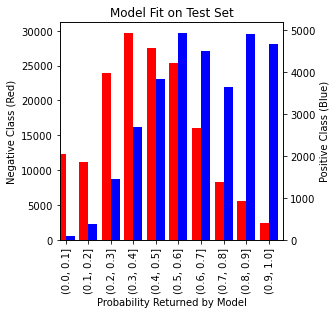
\includegraphics[scale=0.8]{Model_Probabilities_by_Class.png}
\end{center}

By default, one uses a threshold $Pr = 0.5$ to assign the samples to the negative (majority, $Pr < 0.5$) or positive (minority, $Pr > 0.5$) classes, but we are free to change that threshold.  In the bar graph, all red elements to the left of the threshold are TN, all red elements to the right are FP, all blue elements to the left are FN, and all blue elements to the right are TP.  The threshold is a hyperparameter that affects all of the above metrics; for example, decreasing the threshold would shift samples from TN to FP, and from FN to TP.   Decreasing the threshold would over-predict the minority class, and increasing it would under-predict.  

The chart below gives metrics on that model on the CRSS dataset for different thresholds $t$.  The last column is the marginal tradeoff between unneeded ambulances sent and needed ambulances not sent; for instance, at threshold $p = 0.50$, the difference between $p = 0.45$ and $p = 0.55$ is 5.99 ambulances unnecessarily sent for every needed ambulance not sent.  If we (as a society) believe that that cost is too high and we should send fewer ambulances, we should choose a larger threshold value and under-predict the minority class.  For the purposes of this paper we have arbitrarily chosen 10 as the number of additional false alarms we are willing to tolerate for each additional ambulance sent when needed, so we could change the threshold to somewhere in $0.3 < t < 0.4$, over-predicting the minority class.

% From CRSS_07_01_22_ROC_Curves
\begin{center}
\begin{tabular}{r*8{|r}}
	\multicolumn{1}{c|}{$t$}  & \multicolumn{1}{c|}{TN} & \multicolumn{1}{c|}{FP} & \multicolumn{1}{c|}{FN} & \multicolumn{1}{c|}{TP} & \multicolumn{1}{c|}{TPR} & \multicolumn{1}{c|}{FPR} & 
	$\displaystyle \frac{ \Delta \text{TPR}}{\Delta \text{FPR}}$ &
	$\displaystyle \frac{ \Delta \text{FP}}{\Delta \text{TP}}$ \vrule width 0pt depth 12pt \cr\hline
	0.00 & 0 & 162200 & 0 & 31083 & 1.00 & 1.00 & 0.02 & 246.76 \cr
0.10 & 12322 & 149878 & 84 & 30999 & 1.00 & 0.92 & 0.09 & 58.08 \cr
0.20 & 23556 & 138644 & 455 & 30628 & 0.99 & 0.85 & 0.26 & 20.33 \cr
0.30 & 47541 & 114659 & 1895 & 29188 & 0.94 & 0.71 & 0.37 & 14.10 \cr
0.40 & 77254 & 84946 & 4590 & 26493 & 0.85 & 0.52 & 0.60 & 8.74 \cr
0.50 & 104764 & 57436 & 8425 & 22658 & 0.73 & 0.35 & 0.87 & 5.99 \cr
0.60 & 130098 & 32102 & 13362 & 17721 & 0.57 & 0.20 & 1.23 & 4.25 \cr
0.70 & 146094 & 16106 & 17860 & 13223 & 0.43 & 0.10 & 1.77 & 2.95 \cr
0.80 & 154351 & 7849 & 21506 & 9577 & 0.31 & 0.05 & 3.09 & 1.69 \cr
0.90 & 159855 & 2345 & 26404 & 4679 & 0.15 & 0.01 & 8.00 & 0.65 \cr
1.00 & 162200 & 0 & 31083 & 0 & 0.00 & 0.00 & 14.18 & 0.37 \cr

\end{tabular}
\end{center}

%%%
\subsubsection{Area Under the ROC Curve [Needs Citations]}

The Receiver Operating Characteristic (ROC) shows how much the positive and negative classes are interleaved.  It is a parameterized curve following the probability threshold from $t=0$ to $t=1$, and plotting the true positive rate (TPR) versus the false positive rate (FPR).  The orange ``Model''  curve in the graph below is from the same dataset predictions in the chart above.  The eleven points correspond to the (FPR,TPR) coordinates in the chart, going from $t=0.0$ in the upper right to $t=1.0$ in the lower left.    The next-to-last column in the chart gives the slope of the ROC curve.  

If the model gave entirely random results, the bars in the bar chart above would all have the same height (1/20 of the number of elements in the class), and the slope of the ROC curve would be 1, illustrated by the green line, and the area under the curve (AUC) would be $0.5$.  If our model and dataset were ideal, with all of the negative elements having $Pr=0.0$ and all of the positive elements having $Pr=1.0$, the ROC curve would be the blue $\Gamma$, with area under the curve of 1.0.  In practice, the area under the curve is between 0.5 and 1.0.  

The area under the ROC curve is useful for comparing different models on the same dataset.  A higher area generally means that the model more clearly separates the two classes, and is more likely to correctly classify elements of a different (but related) set of samples.

Because both TPR and FPR are unaffected by class imbalance, the ROC curve is as well.  



\begin{center}
	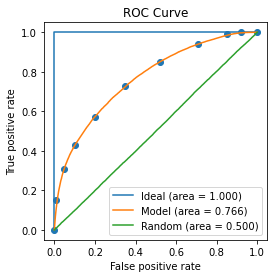
\includegraphics[scale=0.8]{ROC_Example.png}
\end{center}
